\documentclass[svgnames]{beamer}


\mode<presentation>
{
  \usetheme[titleformat=smallcaps,numbering=fraction,progressbar=frametitle]{metropolis}
  \usecolortheme[light,accent=orange]{solarized}
  %\usecolortheme[named=Goldenrod]{structure}
  % or ...

  \setbeamercovered{transparent}
  % or whatever (possibly just delete it)
}


% \usepackage{mathtext}
\usepackage[utf8]{inputenc}
\usepackage[english,russian]{babel}
\usepackage{cmap}
\hypersetup{unicode=true}
\graphicspath{{images/}{slides/images}}


\title[CTA 01] % (optional, use only with long paper titles)
{Слова — Лексическая статистика}

\subtitle
{Квантитативный анализ текста} % (optional)

\author%[Author, Another] % (optional, use only with lots of authors)
{Кирилл Александрович Маслинский}
% - Use the \inst{?} command only if the authors have different
%   affiliation.

\institute%[Universities of Somewhere and Elsewhere] % (optional, but mostly needed)
{Институт русской литературы (Пушкинский Дом) РАН}
% - Use the \inst command only if there are several affiliations.
% - Keep it simple, no one is interested in your street address.

\date%[Short Occasion] % (optional)
{07.02.2022 / 01}

\subject{natural language processing, text mining}
% This is only inserted into the PDF information catalog. Can be left
% out. 



% If you have a file called "university-logo-filename.xxx", where xxx
% is a graphic format that can be processed by latex or pdflatex,
% resp., then you can add a logo as follows:

% \pgfdeclareimage[height=0.5cm]{university-logo}{university-logo-filename}
% \logo{\pgfuseimage{university-logo}}

% Delete this, if you do not want the table of contents to pop up at
% the beginning of each subsection:

\newcommand{\plate}[1]{\begingroup\setbeamercolor{background canvas}{bg=Beige}
  % \begin{frame}<beamer>{Outline}
  %   \tableofcontents[sectionstyle=show/hide,subsectionstyle=show/shaded/hide]
  % \end{frame}
  \begin{frame}[plain]
  \vfill
  \centering
  \begin{beamercolorbox}[sep=8pt,center,shadow=true,rounded=true]{title}
    \usebeamerfont{title}#1\par%
  \end{beamercolorbox}
  \vfill
  \end{frame}
  \endgroup
}

% \AtBeginSection[]
% {
%   \begin{frame}<beamer>[plain]{План}
%     \tableofcontents[sectionstyle=show/hide,subsectionstyle=show/shaded/hide]
%   \end{frame}
% }

\AtBeginSubsection[]
{
  \begin{frame}<beamer>[plain]{План}
    \tableofcontents[sectionstyle=show/hide,subsectionstyle=show/shaded/hide]
  \end{frame}
}

\newcommand{\tb}[1]{\colorbox{yellow}{#1}\space}
\newcommand{\Sp}[1]{\colorbox{green}{#1}\space}
\newcommand{\Sn}[1]{\colorbox{red}{#1}\space}


\begin{document}

\begin{frame}
  \titlepage
\end{frame}

\begin{frame}[plain]
  \centering
  \Huge\bfseries
  \structure{Предисловие}
\end{frame}


\begin{frame}
  \centering
  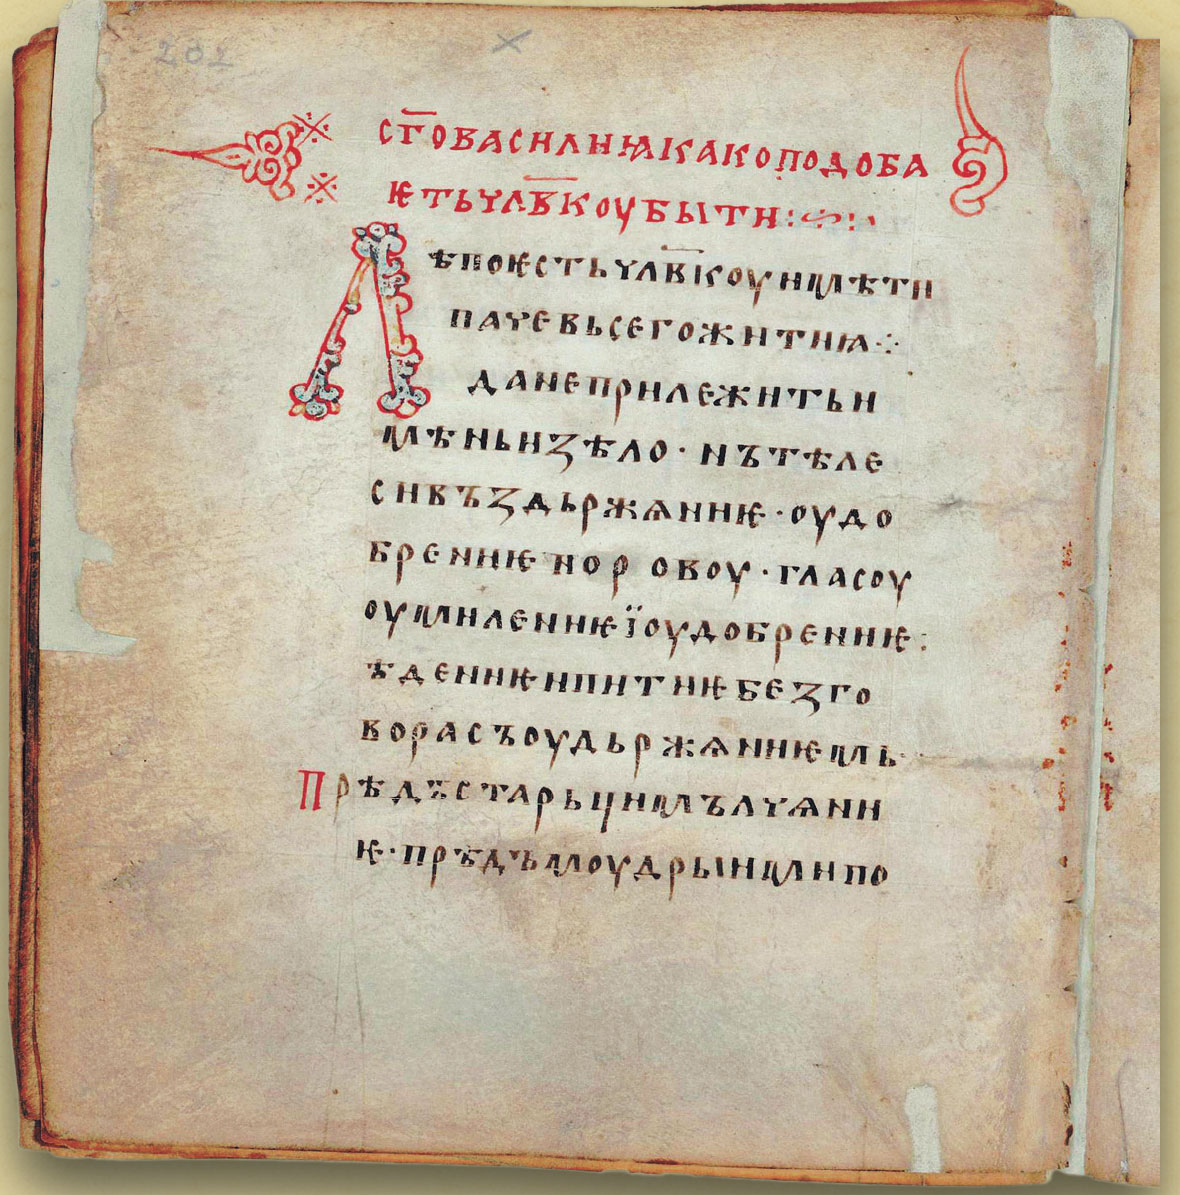
\includegraphics[height=.95\textheight]{izbornik1076}
\end{frame}

\begin{frame}[standout]
  When Irish monks began separating words in manuscripts
by spaces in the seventh century, little could they know
that they were performing a central task of computational
text analysis.

\textit{Andrew Piper, Enumerations: Data and literary study (2018) p. 42}
\end{frame}

\section{Лексическая статистика}

\begin{frame}
  \frametitle{Как начать считать слова}
  \begin{itemize}[<+->]
  \item сколько разных слов в сообщении в
    мессенджере?
  \item на странице научной статьи?
  \item сколько новых слов на каждой следующей
  странице,
  \item сколько новых слов во второй половине книги (по
    сравнению с первой)?
  \item сколько новых слов в книге по сравнению
  с другими книгами? 
  \item когда наконец мы перестанем встречать новые слова?
  \end{itemize}
\end{frame}

\subsection{Закон Ципфа}

\begin{frame}[plain]
  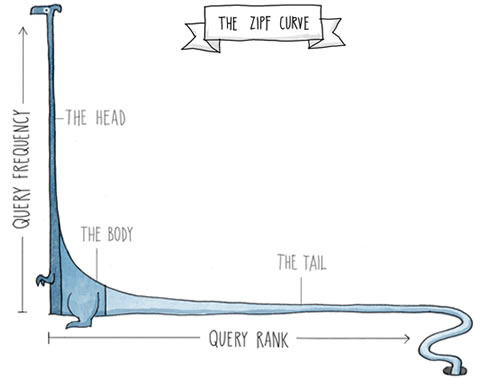
\includegraphics[width=\textwidth]{zipf-animal}
\end{frame}

\begin{frame}
  \frametitle{Закон Ципфа}
  \framesubtitle{Zipf's law (1949)}
  Предсказывает частотность слова по его рангу в частотном списке:
    \begin{equation}
      f(w) = \frac{C}{r(w)^a}
    \end{equation}
    \begin{itemize}
    \item[$f(w)$] — частотность слова $w$
    \item[$r(w)$] — ранг слова $w$ в частотном списке
    \item[$C$] — константа
    \item[$a$] — константа, близкая к 1.
    \end{itemize}
\end{frame}

\begin{frame}
  \frametitle{Предсказания закона Ципфа}
  При \structure{$a=1$}, \structure{$C=60000$} закон Ципфа предсказывает:
  $$
       f(w) = \frac{C}{r(w)}
  $$
 \begin{itemize}
  \item самое частотное слово встретится $f(w)=C/1=60000$ раз
  \item второе по частотности слово $C/2=30000$ раз
  \item третье по частотности слово $C/3=20000$ раз
  \item сотое $C/100=600$ раз
  \item сто первое $C/101=594,06$ раз (около 99\% частотности сотого)
  \item и длинный хвост из 80000 слов с частотностью между $1,5$ и $0,5$.
  \end{itemize}
\end{frame}

\begin{frame}
  \frametitle{Логарифмическая форма закона Ципфа}

  \begin{columns}
    \column{.55\textwidth}
    \begin{equation}
      \log f(w) = log(C) - a\log r(w)
    \end{equation}

    \begin{block}{Линейная функция:}
    $$
    y = kx + b
    $$
  \end{block}
    \column{.45\textwidth}
\end{columns}
\end{frame}

\begin{frame}[plain]
  
\includegraphics[width=\textwidth]{zipf-log-ex}
\end{frame}

\begin{frame}
  \frametitle{Закон Ципфа-Мандельброта (1953)}
  \begin{equation}
    f(w) = \frac{C}{(r(w) + \alert{b})^a}
  \end{equation}
  При \structure{$C=60000$}, \structure{$a=1$}, \structure{$b=1$}
  предсказанная частотность самого частотного слова:
  \begin{description}
  \item[Закон Ципфа] $\frac{C}{1}=\frac{60000}{1}=60000$
  \item[Закон Ципфа-Мандельброта] $\frac{C}{r+b}=\frac{60000}{(1+1)}=30000$
  \end{description}
\end{frame}


\begin{frame}
  \frametitle{Объяснения закона Ципфа}
  \begin{enumerate}
  \item Психолингвистическое (Ципф):
    \begin{itemize}
    \item экономия усилий говорящего (меньше разных слов);
    \item экономия усилий слушающего (больше разных слов).
    \end{itemize}
  \item Теоретико-информационное (Мандельброт):
    \begin{itemize}
    \item минимизация средней стоимости передачи информации в тексте.
    \end{itemize}
  \item Процесс, приводящий к подобному распределению:
    \begin{itemize}
    \item новые слова с константной вероятностью (Simon 1955);
    \item «обезьяна и пишущая машинка» (Miller 1957).
    \end{itemize}
  \end{enumerate}
\end{frame}


\begin{frame}
  \frametitle{Степенное распределение}
  
  Few Giants — Many dwarfs

  \begin{block}{Примеры}
  \begin{itemize}
  \item частотности слов;
  \item размеры городов;
  \item распределение дохода (закон Парето).
  \end{itemize}    
  \end{block}
\end{frame}

\subsection{Частотность и состав лексикона}

  \begin{frame}
    \frametitle{Открытые и закрытые классы слов}
      Словарь языка незамкнут — всё время возникают новые слова.
    \begin{description}
    \item[Function words, closed-class] 
      Вершину частотного списка занимают служебные части речи
      (\alert{предлоги, союзы, местоимения}). Все единицы перечислимы,
      пополняется очень медленно. В тексте выполняют прежде всего
      грамматическую функцию. 
    \item[Content words, open-class]
      Далее в частотном списке преобладают слова открытых классов (пополняемых), прежде
      всего \alert{существительные}. В тексте выполняют прежде всего
      референтную функцию.
    \end{description}
  \end{frame}


\begin{frame}[fragile]
  \frametitle{Пример: частотность русской лексики}
  Единица измерения частотности:
  \begin{itemize}
  \item[ipm] — вхождений на миллион / instances per million 
  \end{itemize}
  \small
  \begin{columns}
    
\column{.5\textwidth}
\begin{verbatim}
1 36358.94 и misc 
2 27792.36 в prep 
3 20689.51 не misc 
4 18942.62 он pron 
5 16588.14 на prep 
6 15631.11 я pron 
7 12546.08 что misc 
8 11398.44 тот adjpron
9 11223.99 быть verb 
10 11150.72 с prep 
11 9808.61 а misc 
12 8604.72 весь adjpron
13 8043.90 это pron 
14 7313.35 как misc 
15 7110.80 она pron 
\end{verbatim}
\column{.5\textwidth}
\begin{verbatim}
32600 1.04 мертветь verb
32601 1.04 сволочной adj
32602 1.04 втыкаться verb
32603 1.04 нахлебник noun
32604 1.04 русоволосый adj
32605 1.04 автопилот noun
32606 1.04 иссечение noun
32607 1.04 бульдожий adj
32608 1.04 бренность noun
32609 1.04 нездоровье noun
32610 1.04 саргасса noun
32611 1.04 коротковатый adj
32612 1.04 кукурузник noun
32613 1.04 шарлатанство noun
32614 1.04 селекционер noun
\end{verbatim}
  \end{columns}
\end{frame}
  

\subsection{Размер и скорость роста словаря}


\begin{frame}
  \frametitle{Скорость роста словаря}
  Чем дальше мы читаем текст, тем реже встречаем новые слова.

  Оценка Гаральда Баайена (Baayen G):
  \begin{equation}
    G = \frac{V(1)}{N}
  \end{equation}
где: 
\begin{itemize}
\item[$V(1)$] — количество hapax legomena на $N$ токенов текста
\item[$N$] — количество токенов текста.
\end{itemize}
\end{frame}

\begin{frame}
  \frametitle{Рост словаря}
  \framesubtitle{Vocabulary growth}
  Чем дальше мы читаем текст, тем реже встречаем новые слова.
  \begin{columns}
    \column{.5\textwidth}
    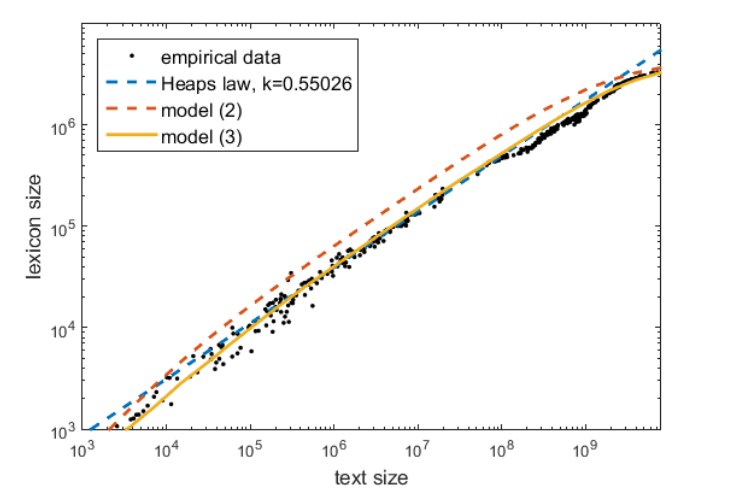
\includegraphics[width=\textwidth]{heaps-law}
    \column{.5\textwidth}
  \begin{equation}
    V = kN^{\beta}
  \end{equation}
  \begin{itemize}
  \item[$V$] — размер словаря
  \item[$N$] — размер корпуса
  \item[$k$] — константа (обычно 10—100)
  \item[$\beta$] — константа $0 < \beta < 1$ (обычно 0,4—0,6)
  \end{itemize}
  \end{columns}
\end{frame}

\begin{frame}
  \frametitle{Probability to see a word}

  Maximum Likelihood Estimation (MLE) — based on the observed
  frequency in the corpus:

  $$
  P = \frac{f(w)}{N}
  $$
  где 
  \begin{itemize}
  \item[$P$] — probability;
  \item[$f(w)$] — word frequency $w$;
  \item[$N$] — corpus size.
  \end{itemize}
\end{frame}

\begin{frame}
  \frametitle{Probability to see a word}

  Model Based Estimation (LNRE model) — based on the knowledge of the
  general properties of word distributions:

  $$
  P = \frac{C}{(r(w) + b)^a}
  $$
  \begin{itemize}
  \item[$P$] — probability;
  \item[$f(w)$] — word rank $w$ in a frequency list;
  \item[$a$, $b$] — model parameters;
  \item[$C$] — normalizing constant.
  \end{itemize}

  This is Zipf-Mandelbrot model
\end{frame}

\subsection{Размер лексикона/Лексическое разнообразие}

\begin{frame}
  \frametitle{Коэффициент лексического разнообразия}
  \framesubtitle{Type/token ratio}
  Одна из первых и широко используемых мер сложности речи/текста.
  \begin{equation}
    TTR = \frac{V}{N}
  \end{equation}
  \begin{itemize}
  \item[V] — размер словаря, число разных словоформ/лемм в тексте (types)
  \item[N] — число словоформ в тексте
  \end{itemize}
  \pause
  Обратная величина: средняя частотность слов в тексте
  \begin{equation}
    F_{mean} = \frac{N}{V}
  \end{equation}
\end{frame}

\begin{frame}
  \frametitle{TTR: проблемы}
  Классические применения:
  \begin{itemize}
  \item определение авторства
  \item оценка сложности (детской) речи — развития речи
  \end{itemize}
  Проблемы:
  \begin{itemize}
  \item \alert{зависит от длины текста}, длиннее текст — ниже TTR (r=0.99).
  \item зависит от способа выделения types (словоформы/леммы)
  \end{itemize}
  Нормализованная версия TTR:
  \begin{itemize}
  \item для сравнения используются фрагменты текста одинаковой длины.
  \end{itemize}
\end{frame}

\subsection{Практические следствия закона Ципфа}

\begin{frame}
  \frametitle{Практические следствия закона Ципфа}
  \begin{enumerate}
  \item \alert{Data sparseness} — в сколь угодно большом корпусе:
    \begin{itemize}
    \item почти все слова встречаются очень редко;
    \item небольшая группа частотных слов составляет значительную
      часть токенов корпуса;
    \item LNRE — Large Number of Rare Events. 
    \end{itemize}
  \item \alert{Рост словаря} — даже очень большие корпуса не содержат всех слов языка:
    \begin{itemize}
    \item искаженная оценка вероятности слова по частотности в корпусе;
    \item нельзя использовать размер словаря для оценки степени
      лексического разнообразия текста.
    \end{itemize}
  \item \alert{Знания о распределении} слов в любом тексте можно использовать
    для оптимизации и построения моделей.
  \end{enumerate}
\end{frame}

\section*{Заключение}

\begin{frame}
  \frametitle{Takeaways}
  \begin{itemize}
  \item Помни о словах, которые еще не встретились. Делай на них
    \textbf{скидку}. 
  \item Никогда не суди о богатстве словаря автора по количеству разных слов в
    тексте. 
  \item Откинув небольшое число самых частотных слов, можно резко
    сократить объем корпуса, сохранив б\'{о}льшую часть смысловых слов.
  \end{itemize}
\end{frame}
\end{document}
